\chapter{Conclusion}

\section{Summary}

To summarise this thesis,~\gls*{mcrt} is a powerful technique that can be used to calculate the transport of light (as particles or quasi-wave/particles) through turbid media, whilst modelling multiple anisotropic scattering alongside a variety of microphysics.
The only noted downsides to the~\gls*{mcrt} method noted in the literature (as well as discussed at length in this thesis) is the computational load required for some problems and the optical properties.
With the growing computational power year on year, more and more the computational load of \gls*{mcrt} becomes less of a factor.
Likewise the optical properties of various biological tissues, are increasing being measured with greater precision and accuracy.

\medskip

Chapter 1 introduced the concept at the heart of this thesis, the Monte Carlo method.
The chapter gave examples of how the Monte Carlo method can be used to sample from spectra, and how it is used to model various physical events.
Chapter 2 followed on from chapter 1 explanation of the Monte Carlo method, by introducing \gls*{mcrt} used in all subsequent chapters.
Chapter 2 covered the theory behind the method and presented details of the implementation into code alongside various computational speedups.

\medskip

Chapter 3 described the application of the \gls*{mcrt} method to modelling tissue ablation.
Details of how the \gls*{mcrt} was coupled up to a numerical model of heat diffusion and thermal damage model was presented.
The chapter showed that we can successfully model experimental and theoretical data with our numerical model.
The power the model has is that we can predict thermal damage, and ablation crater size for any laser, and configuration thereof, without the need to test on humans or animals.
It also allows the testing of different lasers without the purchase of said laser, which could allow clinicians to ``try before they buy''.
The chapter also presented (with tongue firmly in cheek) the application of this numerical model to humane spy disposal.

\medskip

Chapter 4 presented the modification of the \gls*{mcrt} method, such that it would allow the modelling of the photon packets as quasi-wave/particle packets, in place of the usual particle model \gls*{mcrt} models.
This was achieved via a few small changes within the code, based upon well understood theoretical models, namely the Fresnel-Huygens principle.
The method was thoroughly validated against several theoretical expressions.
The method was the validated against experimental results from collaborators at the University of Dundee.
The new method was then used to compare Bessel and Gaussian beams performance in highly turbid media.
The method showed that blah

\medskip

Chapter 5 presented a model of skin autofluorescence using \gls*{mcrt}.
The chapter detailed a five layer skin model created to accurately model the skin effect on light transport.
The five layer model included the various chromophores found in the skin such as blood, water, and melanin.
The model also includes various naturally occurring fluorophores.
Changes in the autofluorescent response of tissue has been shown to be indicative of various diseases.
Therefore the \gls*{mcrt} algorithm was coupled to an optimisation technique to determine relative concentrations of the fluorophores in the skin.
The technique chose was the Nelder-Mead method.
The \gls*{nm} method uses simplices in order to move around the search space and find global minima.
The method was coupled to the the MCRT algorithm and thoroughly validated against toy models.
Finally details of how autofluorescent data from collaborators was fitted using these techniques.

\medskip

Finally chapter 6 presented ...

\section{Future Prospects}

There are several avenues of promising work that can continue on from this thesis.

One obvious avenue of future research would be to improve the five layer skin model presented as part of chapter 5 work.
The skin model presented is planar, where as tissue is not planar in any sense.
The first improvement on this could be to introduce a more complex geometrical structure into the voxel model.
However, this method would quickly run into a computational wall.
To represent the non planar reality if the tissue would require many voxels, such that the RAM required to run any simulation would be prohibitive to running the simulations.
Therefore, a different geometrical model would need to be used.
A solution to this was briefly investigated: use of a mesh to model the skin's structure.
Triangular meshes can be used to model any arbitrary shape or volume [cite].
The use of triangular meshes have been used to great effect by other authors in \gls*{mcrt} codes.
Due to time constraints this was abandoned for this thesis before a fully working code could be developed.
\Cref{fig:mesh} shows \gls*{mcrt} being preformed on a gourd, made from a triangular mesh.

\begin{figure}[!htpb]
    \centering
    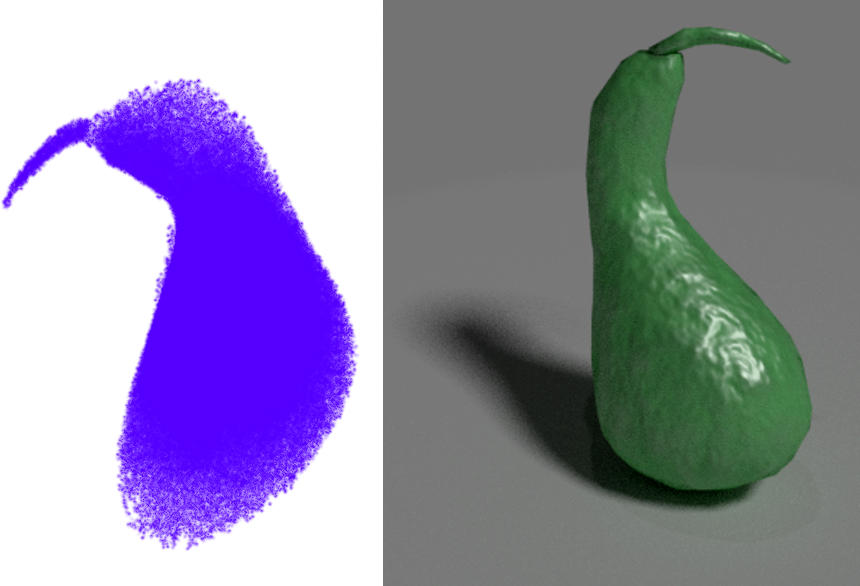
\includegraphics[width=0.5\textwidth]{gourd-fluence.png}
    \caption{Image on the left shows the fluence of light in a gourd, calculated using \gls*{mcrt}. The optical properties of the gourd in this simulations are similar to that of skin. The optical properties of the medium around the gourd are that of air. Image on the right shows a rendering of the same mesh in blender.}
    \label{fig:mesh}
\end{figure}

The code developed as part of the tissue ablation chapter, could easily be adapted for use in modelling photothermal therapy.
Photothermal therapy is the use of light to selectively heat up nanoscale material that have been inserted into tumours (which preferentially accumulate in the tumors).
The nanoscale materials, such as gold nanorods, are targeted with a specific wavelength of light (usually infra-red) which heats up the rods and thus the surrounding tissue, eventually killing the adjacent cells.
This could be easily modelled within the code developed as art of chapter 3.
The code could be used to help optimise treatment modalities and predict treatment outcomes. ***sources***

The work of chapter 3 could also be extended to include a drug diffusion model.
This would allow the simulation of how topical drug diffusion into the skin can be assisted by using laser beams to optically drill channels into the skin to promote drug diffusion.

chapter 4 work could be extended to model speckle imaging + wavefront shaping?


chapter 5 could use other optimisation techniques GA simulated annealing

